\chapter{Pengenalan Algoritma dan Pemrograman}\label{ch:pengantarAlgoritma}

%
%- Pengantar
%- Permasalahan
%- Algoritma
%- Peran Pemrograman Pada ALgoritma
%- Konsep Algorima dan Pemrograman Dasar
%/// PENGAYAAN
%- Kontes
%

\section{Pengantar}

\newthought{Teknologi Informasi semakin berkembang pesat setiap saat}, hal tersebut bisa dilihat dari munculnya perangkat-perangkat keras seperti \textit{smart phone}, PC, \textit{notebook} dan gadget lainnya. Perangkat-perangkat tersebut tidak berguna tanpa adanya berbagai perangkat lunak (aplikasi) yang berjalan di dalamnya. Perangkat-perangkat lunak tersebut terdiri dari berbagai jenis, antara lain seperti: perangkat lunak sistem operasi (contoh Windows, Linux, Android, iOS dan lain-lain) yang merupakan fondasi dari aplikasi-aplikasi lain serta perangkat lunak perkantoran seperti \textit{text processor} atau \textit{spreadsheet}, kalender, reminder, penghemat baterai, penghapus berkas (\textit{file}) tidak berguna dan lain-lain. 
 
\begin{marginfigure}
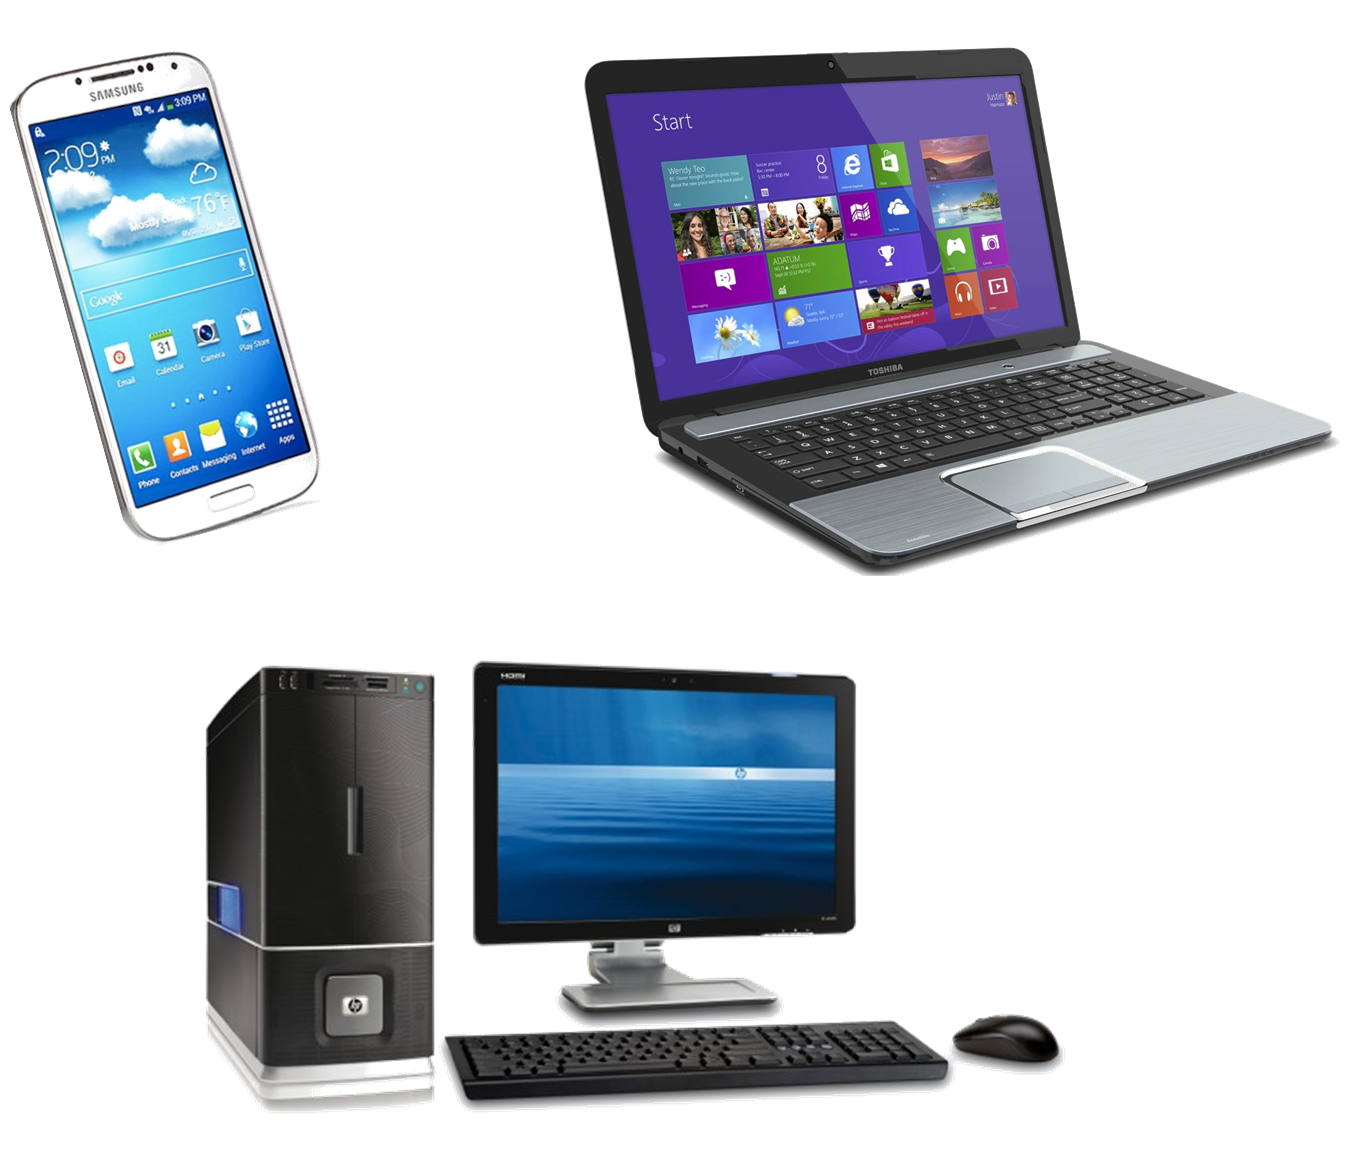
\includegraphics[scale=0.3]{fig/1/Gambar1.png}
\caption{Gadget di Era Modern}
\label{fig:gadgetModern}	
\end{marginfigure}

Jika dilihat dari sudut pandang tertentu, sebuah aplikasi pada dasarnya dibuat untuk menyelesaikan masalah. Kita ambil sebuah contoh misalnya, sebuah aplikasi \textit{spreadsheet} yang sudah sering kita gunakan yaitu \textit{Microsoft Excel}. Aplikasi ini dapat menyelesaikan banyak masalah mulai dari masalah perhitungan sederhana, logika, statistik, sampai pada pembuatan laporan keuangan yang kompleks \footnote{Bisakah anda memikirkan aplikasi lain yang bisa memecahkan masalah anda?}
. Contoh lain adalah aplikasi permainan yaitu: Poker. Apakah ada masalah yang diselesaikan oleh aplikasi permainan Poker? Ternyata, walaupun aplikasi Poker hanya merupakan aplikasi permainan, akan tetapi dibalik aplikasi tersebut banyak masalah-masalah yang harus diselesaikan agar dapat dinikmati seperti misalnya: proses pengacakan kartu, pembagian kartu, pengecekan kemenangan kartu, serta bagaimana agar pihak komputer (AI) lebih mahir bermain daripada \textit{player}. Poker tentu tidak akan menyenangkan jika ternyata pada pembagian kartu, terdapat kartu yang berulang, proses pembagian kartu yang tidak acak/berulang-ulang, dan pembayaran hadiah kemenangan yang salah. Kesimpulannya, untuk mengembangkan sebuah aplikasi yang bagus diperlukan banyak proses pemecahan masalah didalam aplikasi tersebut.

Dari narasi di atas, muncul pertanyaan seperti:
\begin{enumerate}
	\item Bagaimana perangkat lunak dapat menyelesaikan masalah?
	\item Apakah ada sebuah entitas cerdas di dalamnya yang menyelesaikan masalah dan beradaptasi pada setiap permintaan-permintaan pengguna?
\end{enumerate}
  
Jawaban dari pertanyaan tersebut berkaitan dengan bagian dari perangkat lunak yaitu algoritma. Kita ambil contoh, misalnya pada program \textit{Microsoft Excel}, proses penggunaan rumus-rumus memiliki algoritmanya sendiri, proses membuatan laporan memiliki algoritmanya sendiri dan seterusnya. Demikian juga pada aplikasi permainan Poker, proses pengacakan memiliki algoritmanya sendiri, proses pengecekan kemenangan memiliki algoritmanya sendiri dan seterusnya. Sampai disini kita tahu bahwa, sebuah perangkat lunak selain menyelesaikan banyak masalah juga terdiri dari banyak algoritma (jika masalah yang diselesaikan semakin banyak) dan algoritma adalah sesuatu yang digunakan untuk menyelesaikan masalah.


\section{Pengertian Algoritma dan Masalah}
Sebelum kita membahas lebih lanjut mengenai algoritma, alangkah baiknya kita memahami lebih lanjut mengenai apa itu ``masalah''. Jika sebelumnya diceritakan mengenai masalah dari sisi perangkat lunak, pada bagian ini kita akan melihat masalah pada kehidupan sehari -hari. 

\subsection{Permasalahan}
Coba perhatikan berbagai masalah kehidupan sehari-hari berikut ini:

\begin{enumerate}
	\item Anda diminta untuk menyusun voucher-voucher berikut ini menjadi terurut, sehingga pihak panitia akan mudah melakukan tracking terhadap voucher yang sudah masuk.  
	
\begin{center} \large
  \begin{tabular}[h!]{| c | c | c | c | c | c | c | c | c | c | }
	\hline
    10 & 3 & 8 & 5 & 9 & 2 & 1 &  7 & 4 & 6 \\
	\hline
  \end{tabular}
\end{center}

	\item Anda diminta untuk mencari apakah NIM 141112020 merupakan peserta ujian ? 
		\large
			\begin{center}
				\begin{tabular}[h!]{| c | c |}
				\hline
				\multicolumn{2}{|c|}{\textit{PESERTA UJIAN}} \\
				\hline	
				\textit{NIM} & \textit{Nama} \\ \hline
				141110001 & Amir \\ \hline
				141110003 & Budi \\ \hline
				141111111 & Charlie \\ \hline
				141112130 & Dodi \\ \hline
				141113020 & Elsa \\ \hline
				141119191 & Fanny \\ \hline
				141113121 & Gloria \\ 
				\hline
				\end{tabular}
		\end{center}
		
	\item Anda diminta melakukan output pejabat dengan kekayaan tertinggi !
			\begin{center}
				\begin{tabular}[h!]{| c | r |}
				\hline
				\multicolumn{2}{|c|}{\textit{HARTA PEJABAT}} \\
				\hline	
				\textit{Nama Pejabat } & \textit{Jumlah Kekayaan} \\ \hline
				YBS & Rp 19,582,918,419 \\ \hline
				KJ & Rp 19,549,185,718 \\ \hline
				WKJ & Rp 19,527,418,194 \\ \hline
				SP & Rp 19,553,481,751 \\ \hline
				RH & Rp 19,248,572,728 \\ \hline
				WPN & Rp 19,999,999,999 \\
				\hline
				\end{tabular}
		\end{center}
		
\end{enumerate}

Dapatkah Anda memberikan solusi untuk masalah-masalah diatas? Dapatkah anda memikirkan masalah-masalah lain lagi? 

Sepintas melihat pada masalah-masalah diatas, secara langsung kita dapat dengan mudah menemukan solusi untuk masalah-masalah diatas. Ketika masalah bertambah besar atau semakin rumit, kita dipaksa untuk berpikir dan menemukan pola-pola atau langkah-langkah penyelesaian masalah baik secara tertulis ataupun tidak \footnote{Jika masalah semakin besar lagi, terkadang kita memerlukan bantuan komputer.}. Pada akhirnya, proses berpikir atau langkah-langkah yang kita lakukan akan menemukan solusi dari masalah tersebut (atau tidak). 

\subsection{Algoritma}
Proses berpikir atau langkah-langkah menyelesaikan masalah tersebut disebut dengan \textbf{algoritma} \footnote{Cara lain dalam memahami algoritma bisa menggunakan analogi resep memasak. Resep memasak (algoritma) adalah langkah-langkah untuk mencapai suatu hasil masakan (menyelesaikan masalah)}. 

Kata algoritma sendiri berasal dari nama seorang matematikawan Persia (sekarang Iraq) yaitu Abu Ja`far Mohammed ibn Musa al-Khowarizmi. Al-Khowarizmi sendiri sekarang merupakan sebuah kota Rusia yang bernama Khiva. Dari Al-Khowarizmi diturunkan namanya menjadi Algoritma. 

Dari sisi ilmu komputer, Algoritma merupakan sebuah rangkaian proses komputasional yang mengkonversi satu atau beberapa masukan (\textit{input}) menjadi satu set keluaran (\textit{output}) jika memungkinkan \footnote{Sebuah algoritma juga bisa dilihat sebagai sebuah \textbf{alat} (\textit{tool}) untuk menyelesaikan sebuah \textbf{permasalahan komputasional} tertentu}.

Salah satu contoh lain yang mewakili algoritma adalah masalah \textit{Rubik's Cube} (Gambar \ref{fig:RubikCube}). Di dalam masalah \textit{Rubik's Cube}, sebuah \textit{Rubik's Cube} yang belum terselesaikan adalah sebuah masalah, sebuah \textit{Rubik's Cube} yang sudah selesai adalah solusinya, dan langkah-langkah penyelesaian masalah menjadi solusi adalah algoritmanya. 

\begin{figure*}
	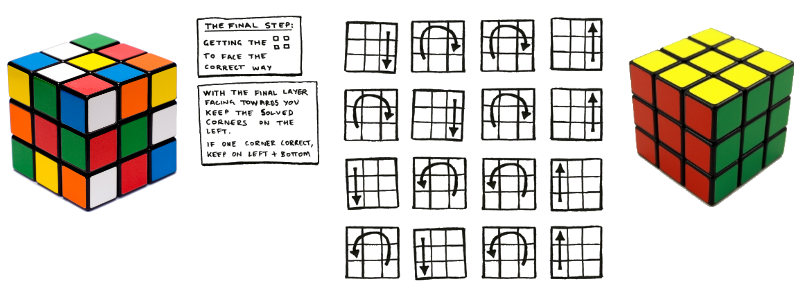
\includegraphics[scale=0.7]{fig/1/Gambar8.png}
	\caption{Permasalahan \textit{Rubik's Cube}. Bisakah anda menemukan langkah-langkah menyelesaikan semua kombinasi di \textit{Rubik's Cube}?}
	\label{fig:RubikCube}
\end{figure*}


Perlu diingat, algoritma yang baik adalah algoritma yang terurut dan efektif.  Perhatikan kasus  dimana kita akan memindahkan isi dari gelas A ke gelas B dengan bantuan gelas kosong C (Gambar \ref{fig:gelasABC}), dapatkah Anda menentukan masalah awal, solusi, dan algoritmanya yang efektif ? Bagaimana jika Anda tidak menjalankan algoritmanya tanpa terurut ? 


\begin{marginfigure}[3cm]
	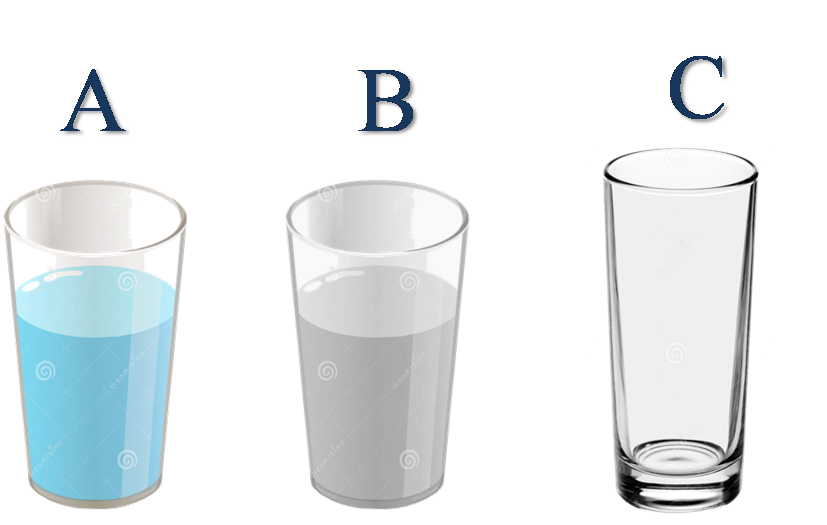
\includegraphics[scale=0.5]{fig/1/Gambar9.png}	
	\caption{Permasalahan pemindahan isi dari Gelas A ke Gelas B dengan bantuan Gelas kosong C}
	\label{fig:gelasABC}
\end{marginfigure}



\subsection{Kenapa harus belajar Algoritma?}
Secara singkat, kita mempelajari algoritma supaya kita bisa menyelesaikan permasalahan-permasalahan komputasional secara \textbf{effisien} \footnote[4.5cm]{Tidak semua permasalahan komputasional bisa diselesaikan secara efisien. Permasalahan yang susah (\textit{Hard Problem}) atau disebut juga permasalahan \textit{NP-complete} masih belum ditemukan algoritma penyelesaian yang effisien.}. Effisien berarti algoritma tersebut memakan waktu dan sumber daya komputasional (mis: memori komputer) yang sedikit. 

Sebagai contoh betapa pentingnya algoritma, kita anggap saja ada dua jenis komputer yang berbeda: A dan B. Komputer A adalah komputer yang sangat cepat dan mampu memproses data sebanyak 10 milyar instruksi dalam 1 detik sedangkan komputer B adalah komputer biasa yang hanya mampu memproses data sebanyak 10 juta instruksi dalam 1 detik. Dengan kata lain, komputer A lebih cepat 1000 kali dari komputer B.

Dari contoh sederhana di atas kita bisa menarik kesimpulan bahwa algoritma yang baik bisa mengalahkan algoritma yang buruk sekalipun dijalankan di kondisi yang sangat jelek seandainya masukkannya sangat besar sekali. 

Sekarang kita misalkan masing-masing komputer tersebut akan mengurut 10 juta bilangan. Komputer A akan menggunakan algoritma pengurutan X sedangkan komputer B akan menggunakan algoritma pengurutan Y. Algoritma X secara teori tingkat effisiensinya adalah $c_1n^2$ (berarti misalnya untuk setiap 5 bilangan yang diurut, algoritma tersebut memakan waktu $c_15^2 = c_125$ detik, $c_1$ adalah sebuah konstanta yang tergantung pada penerapannya) sedangkan algoritma Y tingkat effisiensinya adalah $c_2n\lg n$. 

Untuk mendramatisir lagi, kita anggap saja algoritma X ditulis oleh programmer yang sangat handal dengan menggunakan bahasa mesin yang sangat effisien sehingga penerapannnya mempunyai tingkat effisiensi $2n^2$ sedangkan algoritma Y ditulis oleh programmer biasa-biasa saja dengan menggunakan bahasa pemrograman yang tidak effisien sehingga penerapannya mempunyai tingkat effisiensi $50n\lg n$.

Sekarang kita bandingkan kedua komputer tersebut ketika mengurut 10 juta bilangan. 
\hspace*{\fill}\\\hspace*{\fill}\\
Komputer A akan memakan waktu:
\hspace*{\fill}\\\hspace*{\fill}\\
$\frac{2\cdot(10^7)^2\ instruksi}{10^{10}\ instruksi/detik} = 20000\ detik\ (5.5\ jam)$
\hspace*{\fill}\\\hspace*{\fill}\\
Sedangkan komputer B akan memakan waktu:
\hspace*{\fill}\\\hspace*{\fill}\\
$\frac{50\cdot10^7lg10^7\ instruksi}{10^{7}\ instruksi/detik} \approx 1163\ detik\ (kurang\ dari\ 20\ menit)$
\hspace*{\fill}\\\hspace*{\fill}\\

\marginnote{\begin{konsep}
Seandainya ada dua jenis algoritma pengurutan, yaitu: \textit{Insertion Sort} dan \textit{Merge Sort}. \textit{Insertion Sort} memerlukan $8n^2$ langkah sedangkan \textit{Merge Sort} memerlukan $64n \lg n$ untuk masukan $n$. Berapakah nilai $n$ dimana \textit{Insertion Sort} mengalahkan \textit{Merge Sort}?
\end{konsep}
}

Kesimpulannya, tujuan mempelajari algoritma adalah sebagai berikut.
\begin{enumerate}
	\item Dari segi praktikal, kita bisa menyelesaikan berbagai permasalahan yang ada dengan menggunakan sekumpulan algoritma yang sudah tersedia. Sebagai contohnya, jika kita ingin mengurut sejumlah bilangan secara menaik/menurun maka kita bisa menggunakan algoritma pengurutan yang tersedia misalnya \textit{Bubble Sort}, \textit{Merge Sort}, \textit{Quick Sort} dan sebagainya. Selain itu, kita juga bisa merancang algoritma baru yang efisien untuk permasalahan yang lebih spesifik lagi.
	\item Dari segi teoritikal, algoritma merupakan bagian terpenting dari pembelajaran Teknik Informatika/Ilmu Komputer. Pembelajaran algoritma sendiri merupakan inti dari Teknik Informatika dan wajib dipahami oleh mahasiswa sebelum mempelajari mata kuliah tingkat lanjutan.
\end{enumerate}


\section{Peran Pemrograman pada Algoritma}

Perhatikan salah satu masalah pengurutan voucher yang sudah kita selesaikan sebelumnya. Anggaplah $S$ merupakan himpunan masalah yang akan kita selesaikan dan $n$ merupakan besar/ruang masalah yang akan diselesaikan.  Untuk kasus Voucher, $S = \left\langle1,2,3,4,5,6,7,8,9,10\right\rangle$ dengan besar masalah adalah $n$ = 10. Dalam kasus tersebut $S$ dan $n$ cukup kecil, sehingga masalah akan cukup mudah diselesaikan oleh manusia dan dengan cepat.

Bagaimana seandainya $S$ merupakan himpunan angka acak yang terdiri dari bilangan bulat 1 sampai 10.000 atau $S = \left\langle1,2, ..., 10000\right\rangle$, dengan besar masalah adalah $n$ = 10.000. Masalah ini bisa diselesaikan oleh manusia, tetapi akan membutuhkan waktu yang lama dan tingkat kesalahan yang tinggi. Dengan perkembangan teknologi saat ini, masalah dengan ruang yang besar dapat diselesaikan dengan kekuatan komputasional (Komputer). Kita bisa merancang sebuah algoritma yang nantinya diterjemahkan menjadi bahasa komputer untuk menyelesaikan masalah tersebut. Adalah tugas seorang programmer untuk menterjemahkan algoritma menjadi bahasa pemrograman.

\subsection{Bahasa Pemrograman}
Ada banyak bahasa pemrograman yang bisa dipelajari \footnote{\url{http://en.wikipedia.org/wiki/List_of_programming_languages}}. Sebagai seorang programmer, haruslah memilih bahasa pemrograman yang cocok dengan dia (bisa dilihat dari kebutuhan dan cara penulisan bahasa pemrograman). Umumnya bahasa pemrograman bisa dibagi atas: 
\begin{enumerate}
	\item \textbf{\textit{Low-Level Programming Language}}, merupakan bahasa pemrograman yang lebih dekat dengan bahasa mesin. Bahasa pemrograman ini masih berupa instruksi-instruksi yang terkadang tidak memiliki arti dengan bahasa manusia normalnya. Contoh \textit{Low-Level Programming Language} misalnya: Assembly, OPCODE dan sebagainya.
	\item \textbf{\textit{High-Level Programming Language}}, merupakan bahasa-bahasa pemrograman yang dibangun diatas Low-Level Programming Language, namun memiliki bahasa yang lebih masuk akal dan lebih bisa dimengerti karena mengikuti kaidah-kaidah bahasa yang ada. Contoh \textit{High-Level Programming Language} misalnya:	Pascal, Ada, Cobol, Basic, Fortran, C, C++, Python dan sebagainya.
	\end{enumerate}

Pada mata kuliah ini, kita akan menggunakan bahasa pemrograman Python \footnote{\url{https://www.python.org/}}\footnote{Silakan baca \url{http://mcsp.wartburg.edu/zelle/python/python-first.html} untuk mengetahui kenapa Python dipilih sebagai bahasa pemrograman yang pertama}. Perlu diingat bahwa, kita bukan mempelajari bahasa pemrograman Python, namun menggunakan Python sebagai alat untuk membantu kita mempelajari penyelesaian masalah melalui pembuatan algoritma dalam bahasa pemrograman.

\subsection{Bahasa Python}

Python memiliki berbagai fitur yang menyebabkan banyak orang memilih python sebagai berikut.
\begin{enumerate}
	\item Cocok untuk pemula
	\\Bandingkan ketiga kode dibawah ini. Manakah yang paling sederhana? 
	\begin{listprog}{Program Hello World dalam C++}
		\label{lst:helloWorldC++}
		\begin{lstlisting}[language=C++]
		#include <iostream>
		using namespace std;
		
		int main{}{
			cout << "Hello World";
			return 0;
		}
		\end{lstlisting}
	\end{listprog}
	\begin{listprog}{Program Hello World dalam Java}
		\label{lst:helloWorldJava}
		\begin{lstlisting}[language=Java]
		public class HelloWorld{
			public static void main(String[] args){
				System.out.println("Hello World");
			}
		}
		\end{lstlisting}
	\end{listprog}
	\begin{listprog}{Program Hello World dalam Python}
		\label{lst:helloWorldPython}
		\begin{lstlisting}[language=Python]
		print("Hello World")
		\end{lstlisting}
	\end{listprog}
	Baik C++ dan Java memerlukan \textit{overhead} dalam listing program mereka seperti misalnya kelas, tipe data, titik koma (;), header, tipe return dan sebagainya. Python sebenarnya juga memiliki semua hal tersebut, tetapi semuanya disembunyikan dalam kesederhanaan bahasa pemrograman. Oleh karena itu, python menjadi pilihan yang tepat bagi mahasiswa ketika mempelajari algoritma tanpa harus terbebani oleh \textit{overhead} listing program yang tidak perlu.
	\item \textit{Python's Integrated Development Environment} (IDLE)
	\\IDLE merupakan lingkungan pemrograman interaktif yang sangat bermanfaat bagi pembelajaran python sendiri. IDLE sudah terinstall secara otomatis ketika menginstall python. Tampilan IDLE bisa dilihat di Gambar \ref{fig:IDLE}. 
	
\begin{figure}
	\centering
		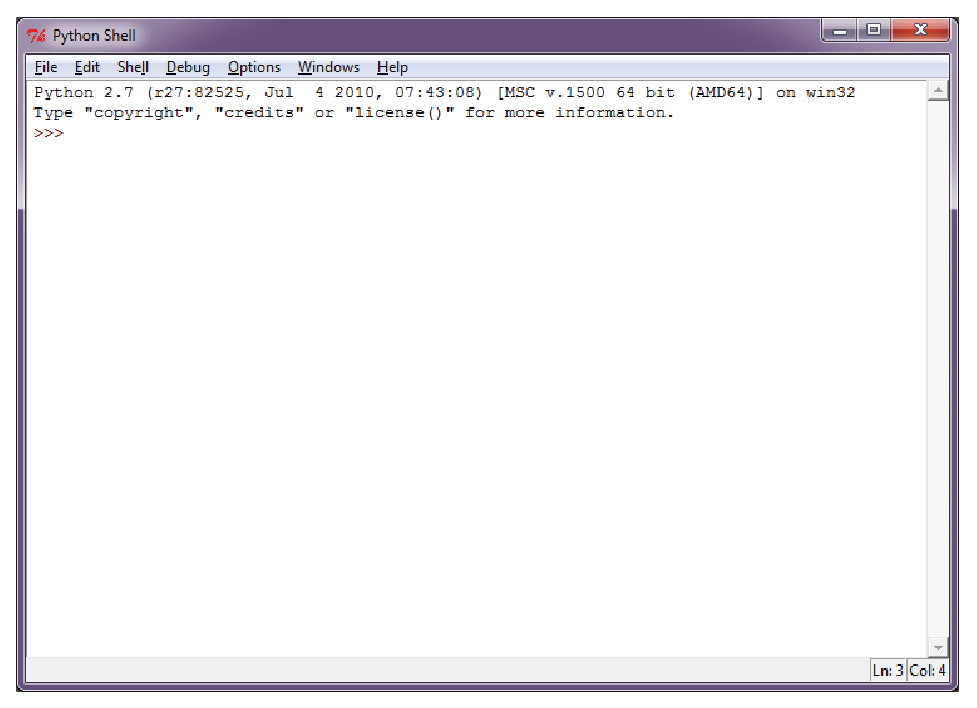
\includegraphics[scale=0.6]{fig/1/IDLE.eps}
	\caption{Tampilan IDLE}
	\label{fig:IDLE}
\end{figure}

	\item Bilangan bulat besar (\textit{Large Integers})
	\\Python sanggup mengatasi \textit{Large Integers} secara \textit{default} dibandingkan dengan bahasa lain (C++, Java dan lain-lain). 
	Contoh jika diketikkan dalam IDLE:
	\begin{IDLE}
	\\$>>>$ 1987163987163981639186L * 198763981726391826L + 23
	\\\textbf{394976626432005567613000143784791693659L}
	\end{IDLE}
	\item Listing program yang bersih dan indah
	\\Listing program yang dituliskan dengan python lebih gampang dibaca. Python secara \textit{default} memaksa programmer untuk membuat program yang lebih terstruktur (paksaan identasi) dan lebih elegan. Program yang ditulis di python bisa lebih pendek daripada Java ataupun C++. 
	 \begin{listprog}{Menulis teks ke file (Java)}
		\label{lst:tulisTeksJava}
		\begin{lstlisting}[language=Java]
		import java.io.*;
		
		public class IOTest{
			public static void main(String[] args) {
		  	try {
		    	File f = new File("scratch");
		      PrintWriter ps = new PrintWriter(new OutputStreamWriter(new FileOutputStream(f)));
					for (int i = 0; i < 1000000; i++) {
						ps.print(String.valueOf(i));
					}
					ps.close();
				}
				catch(IOException ioe) {
					ioe.printStackTrace();
				}
			}
		}
		\end{lstlisting}
	\end{listprog}
	\begin{listprog}{Menulis teks ke File (Python)}
		\label{lst:tulisTeksPython}
		\begin{lstlisting}[language=Python]
		f=open('scratch','wb')
		for i in xrange(1000000):
			f.write(str(i))
		f.close()
		\end{lstlisting}
	\end{listprog}
	\item Dan masih banyak lagi (dynamically typed, lambda, cocok sebagai tool riset dan lain-lain)
\end{enumerate}

Tentunya sebagai bahasa pemrograman pertama yang dipelajari, kita perlu tahu bagaimana menginstalasi Python, menggunakan Python dan menjalankan algoritma pertama kita dengan menggunakan Python. Latihan pada bab ini dapat dikerjakan untuk membantu pemahaman penggunaan Python sebelum masuk ke pemahaman algoritma lebih lanjut. 

\section{Latihan : Pengenalan I}

\begin{pemrograman}
Lakukan langkah-langkah berikut :
\begin{enumerate}
	\item Unduh Python di \url{http://python.org/download/} atau pada E-learning Mikroskil.
	\item Pilihlah python versi 3.3.x \footnote{Versi python (CPython) terdiri dua versi yang digunakan secara umum yaitu versi 2.x.x (yang terbaru adalah 2.7.x) dan 3.x.x (yang terbaru adalah 3.5.x). Keduanya tidak kompatibel, dan ada perbedaan sintaks yang cukup banyak.} yang sesuai dengan OS yang dipakai (Windows 32-bit---Python 3.3.0 Windows Installer, dan Windows 64-bit---Python 3.3.0 Windows Installer). Untuk Linux, python sudah secara \textit{default} terinstall (versi python tergantung dari distro linux yang digunakan).
	\item Install Python Installer yang sudah diunduh.
	\item Buka program \textbf{IDLE} Python yang terinstall bersama Python	
	\item Ketikan \textit{sequence} tersebut di \textbf{IDLE}.
	\begin{IDLE}
	\begin{tabbing}
	$>>>$ print("Hello World")
	\end{tabbing}
	\end{IDLE}
	\item Selain \textbf{IDLE} Python juga memiliki \textbf{IDE (\textit{Integrated Development Environment})} yang bagus seperti PyScripter. Untuk installasi PyScripter cukup unduh dari websitenya \url{https://code.google.com/p/pyscripter/} dan lakukan installasi seperti biasa (harus menginstall python terlebih dahulu).
	\item Buka PyScripter yang sudah diinstallasi, ketikkan Listing \ref{lst:swapSimple} dan jalankan melalui IDE  dengan ketik CTRL-F9.
		\begin{listprog}{Program Swap bilangan (swap.py)}
		\label{lst:swapSimple}
		\begin{lstlisting}[language=Python]
			A = 5
			B = 4
			A = A + B
			B = A - B
			A = A - B
			print(A)
			print(B)
		\end{lstlisting}
\end{listprog}
\end{enumerate}
\end{pemrograman}

\newpage
\section{Pemrograman Kompetitif (\textit{Competitive Programming})}

\newthought{Pemrograman Kompetitif} merupakan kompetisi pemrograman di bidang Teknik Informatika dimana salah satu kompetisi bertaraf Internasional adalah ACM (\textit{International Collegiate Programming Contest}) yang diselenggarakan oleh ACM (\textit{Association for Computing Machinery}\footnote{\url{www.acm.org}}). 

Selain ACM ICPC masih banyak kompetisi serupa yang diadakan baik skala lokal maupun internasional \footnote{STMIK Mikroskil sendiri merupakan satu-satunya partner ACM ICPC untuk menyelenggarakan ACM ICPC Provincial Sumatera di kampus Mikroskil.}, secara offline dan online \footnote{\url{www.topcoder.com}, \url{www.codeforce.com}, dan masih banyak lagi}. 

Tema Pemrograman Kompetitif adalah: ``\textit{diberikan sebuah permasalahan Teknik Informatika, selesaikan dengan secepat mungkin}''. Dalam Pemrograman Kompetitif, mahasiswa bertanding dalam 1 kelompok yang terdiri dari 3 orang dengan hanya 1 komputer. Untuk memenangkan kompetisi Pemrograman Kompetitif, mahasiswa membutuhkan pengetahuan yang mendalam akan algoritma dan telah menyelesaikan soal-soal yang banyak sebelumnya. Kerja sama kelompok yang baik juga merupakan faktor penentu dalam memenangkan kompetisi.

Secara garis besar aturan dan prosedur dari Pemrograman Kompetitif adalah sebagai berikut.
\begin{enumerate}
	\item Peserta membaca soal yang berisikan permasalahan, aturan masukan dan keluaran yang ada.
	\item Peserta kemudian membuat program dengan menggunakan bahasa C++ atau Java untuk menyelesaikan permasalahan dari soal tersebut. Program yang dibuat harus mampu memberikan keluaran sesuai dengan masukan yang ada.
	\item Setelah selesai membuat program, peserta akan mengirimkan \textit{source code} ke sistem judge dari kompetisi. Sistem judge akan menilai apakah keluaran hasil dari program benar atau salah. 
	\item Jika program yang dibuat benar, maka peserta akan melanjutkan mengerjakan soal lain. Jika salah peserta akan memperbaiki program tersebut.
	\item Umumnya kompetisi akan berjalan selama 4-5 jam untuk menyelesaikan 8-10 soal.
\end{enumerate}

Selain mengikuti kompetisi, mahasiswa juga dapat menyelesaikan soal-soal dengan menggunakan \textit{online judge} yang ada seperti:
\begin{enumerate}
	\item \url{uva.onlinejudge.org}
	\item \url{www.spoj.com}
	\item \url{acm.timus.ru}
	\item \url{www.topcoder.com}
	\item \url{www.codeforces.com}\footnote{Website ini merupakan website yang paling sering digunakan untuk berlatih. Selain berlatih, website ini juga memberikan pertandingan online setiap minggu.}
	\item \url{www.codechef.com}
	\item dan sebagainya.
\end{enumerate}

Untuk codeforces, topcoder, dan codechef, website tersebut juga mengadakan kompetisi online setiap pekannya. Mahasiswa diusahakan mengikuti kompetisi online untuk menambah pengalaman kompetisi.

Beberapa topik yang sering diperlombakan di Pemrograman Kompetitif adalah:
\begin{enumerate}
	\item Ad Hoc
	\item \textit{Complete Search (Iterative/Recursive)}
	\item \textit{Divide and Conquer)}
	\item \textit{Greedy}
	\item \textit{Dynamic Programming}
	\item \textit{Graph}
	\item \textit{Mathematics}
	\item \textit{String Processing}
	\item \textit{Computational Geometry}
	\item \textit{Others/Rare problems}
\end{enumerate}

Dari topik-topik tersebut, kebanyakan dibahas di Mata Kuliah Analisis dan Desain Algoritma, tetapi tidak menutup kemungkinan juga mahasiswa mempelajari sendiri topik-topik tersebut secara otodidak melalui Internet.

\newpage
\begin{center}
\textit{Illustrasi soal yang biasa dikeluarkan di ACM-ICPC}\footnote{Penguasaan bahasa Inggris mutlak karena soal yang di kompetisi pemrograman semua menggunakan Bahasa Inggris.}\\
\textbf{Andy\'s First Dictionary}
\end{center}
\hfill\\
Andy, 8, has a dream - he wants to produce his very own dictionary. This is not an easy task for him, as the number of words that he knows is, well, not quite enough. Instead of thinking up all the words himself, he has a briliant idea. From his bookshelf he would pick one of his favourite story books, from which he would copy out all the distinct words. By arranging the words in alphabetical order, he is done! Of course, it is a really time-consuming job, and this is where a computer program is helpful.
\\
You are asked to write a program that lists all the different words in the input text. In this problem, a word is defined as a consecutive sequence of alphabets, in upper and/or lower case. Words with only one letter are also to be considered. Furthermore, your program must be CaSe InSeNsItIvE. For example, words like "Apple", "apple" or "APPLE" must be considered the same.
\\
	\textbf{INPUT}
\\
The input file is a text with no more than 5000 lines. An input line has at most 200 characters. Input is terminated by EOF.
\\
	\textbf{OUTPUT}
\\
Your output should give a list of different words that appears in the input text, one in a line. The words should all be in lower case, sorted in alphabetical order. You can be sure that he number of distinct words in the text does not exceed 5000.
\\
	\textbf{Sample Input}\footnote{Peserta harus membuat program yang bisa membaca input berikut dan mengeluarkan output yang sama persis. Perlu diketahui, input dan output di sini hanya salah satu dari sekian input/output yang nantinya akan diuji oleh judge. Input/output lain dirahasiakan dari peserta.}
\\
\begin{verbatim}	
Adventures in Disneyland

Two blondes were going to Disneyland when they came to a fork 
in the road. The sign read: "Disneyland Left."

So they went home.
\end{verbatim}
\hfill\\
	\textbf{Sample Output}
\\
\begin{verbatim}
a
adventures
blondes
came
disneyland
fork
going
home
in
left
read
road
sign
so
the
they
to
two
went
were
when
\end{verbatim}
\newpage